\section{系统详细设计}
\begin{frame}{架构设计}
    \begin{itemize}
        \item 前端Web界面项目:Vue框架,使用MVVM架构
        \item 后端HTTP服务项目:Tornado + FastAPI框架,使用MVC架构
        \item 软件系统结构:瘦客户机/服务器结构
        \item 系统部署图:
    \end{itemize}
\end{frame}

\begin{frame}{架构设计}
    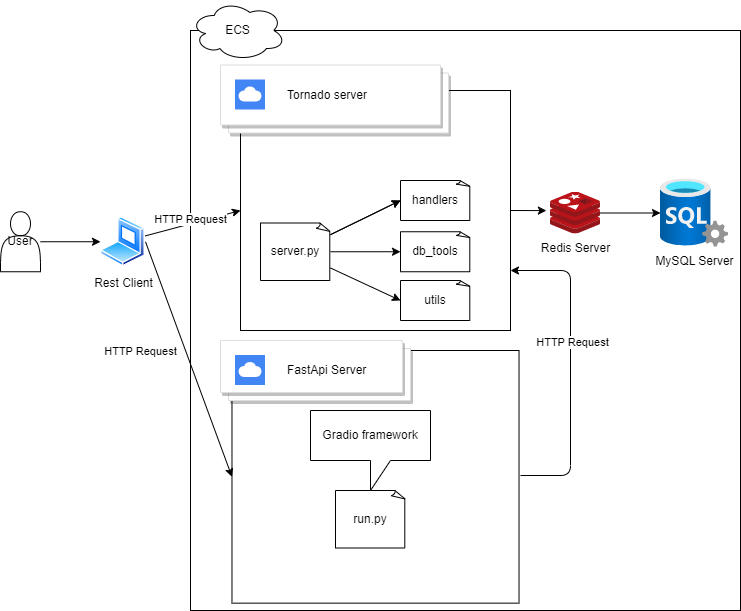
\includegraphics[width=0.8\textwidth]{contents/figure/system_structure.png}
\end{frame}

\begin{frame}
    \frametitle{项目技术栈}
    \begin{itemize}
        \item 主要开发语言:Python
        \item HTTP服务器:Tornado + FastAPI
        \item 前端技术选型:Vue.js + Element UI/HTML + CSS + Js/Gradio
        \item 持久层框架:SQLAlchemy
        \item 数据库服务:MySQL + Redis
        \item 版本管理工具:Git
        \item 远程代码托管平台:华为云
        \item 接口管理与自动化测试工具:Apifox + Mock.js
    \end{itemize}
\end{frame}

\begin{frame}
    \frametitle{项目技术栈}
    \begin{itemize}
        \item AI绘图模型架构:Stable diffusion
    \end{itemize}
\end{frame}

\begin{frame}
    \frametitle{部署说明}
    \begin{itemize}
        \item 需求版本大于等于3.7的Python环境,具有能够支持cuda11.7以上版本cuda toolkit的GPU硬件设备,并且已经正确安装了版本正确的cuda + cudnn
        \item 分别提供了基于Docker和非Docker的部署方式,其中Docker方式需要提前安装好Docker环境
        \item 具体部署流程详见部署指南文档和操作说明,项目启动后软件系统HTTP服务、AI画图服务和后台管理系统服务分别运行在80,8080和7650端口
    \end{itemize}
\end{frame}